\subsubsection{Core Components}
Kubernetes is complex to say the least. However, much of the complexity stems from the control plane which only runs on the master nodes. These nodes are not in the scope of this thesis and thus not explained in more detail. Worker nodes on the other hand are orchestrated and provide their state to the master. This is a lot less resource intensive and there are a few tricks to reduce the resource load even further. But first, for a node to be part of a cluster it needs to run the following components: the \textit{kubelet}, \textit{kube-proxy} and a supported container runtime. How Kubernetes works in practice can be seen in \cref{fig:nodeComponents}\footnote{The \textit{cAdvisor} component is a health checking tool and not required.}.
\begin{figure}[h!]
    \centering
    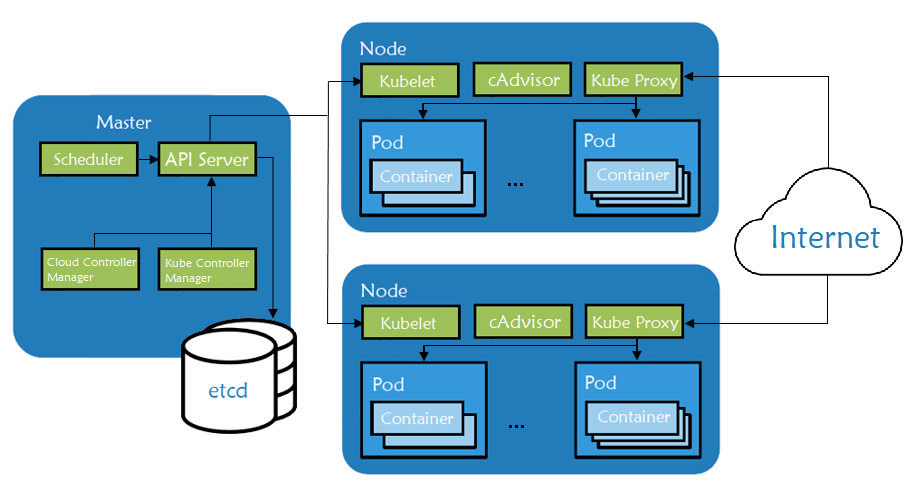
\includegraphics[scale=0.6]{figures/rancherK8sComponents.png}
    \caption{The Kubernetes architecture and node components\cite{nodeSetupKubernetes:online}}
    \label{fig:nodeComponents}
\end{figure}
The kubelet is the primary node agent and schedules and maintains containers running inside a pod based on the pods \textit{PodSpecs}. It gets the these specifications mainly from the APIServer, but other Kubernetes internal sources are possible, too. Containers created outside of Kubernetes are not managed by kubelet. Configuring the kubelet is easily possible via the kubectl and kubeadm tools which give the possibility of enhancing the kubelets performance for different circumstances, here the edge. Going through the possible configurations under \url{https://kubernetes.io/docs/reference/command-line-tools-reference/kubelet/}, the most important configurations for this thesis is the \textit{--housekeeping-interval duration} which defaults to 10s\cite{rancherKubernetesComponents:online}. This means each 10 seconds kubelet performance a complete health check of all its components and sends it to the master. For normal nodes in the cloud, this is fine, but for light edge devices this seems overkill. The k3s kubelet is compatible with Kubernetes and optimized for light edge devices.\\
The kube-proxy is a network proxy node agent ensuring that the Kubernetes networking services runs on each node. It enables the Kubernetes service abstraction by ensuring the network rules on the host and carries out the connection forwarding. The last component, the container runtime, ensures that containers can run as expected. Both components are not from major importance in this thesis.



